%\renewcommand{\theequation}{\theenumi}
%\begin{enumerate}[label=\arabic*.,ref=\thesubsection.\theenumi]
%\numberwithin{equation}{enumi}

\item Find the nature of the roots of the following quadratic equations. If the real roots exist, find them:
\begin{enumerate}
\item 	$2x^2-3x+5 = 0$
\item 	$2x^2-6x+3 = 0$
\item 	$3x^2-4\sqrt{3}x+4 = 0$
\end{enumerate}
\item Solve each of the following equations
%
\begin{enumerate}
\item 	$x^2+3 = 0$
\item 	$2x^2+x+1 = 0$
\item 	$x^2+3x+9 = 0$
\item 	$-x^2+x-2 = 0$
\item 	$x^2+3x+5 = 0$
\item 	$x^2-3x+2 = 0$
\item 	$\sqrt{2}x^2+x+\sqrt{2} = 0$
\item 	$\sqrt{3}x^2-\sqrt{2}x+3\sqrt{3} = 0$
\item 	$x^2+x+\frac{1}{\sqrt{2}} = 0$
\item 	$x^2+\frac{x}{\sqrt{2}}+1 = 0$
\end{enumerate}
%
\item In each of the following exercises, find the coordinates of the focus, axis of the parabola, the equation of the directrix and the length of the latus rectum
\begin{enumerate}
\item $y^2 = 12x$
\item $x^2 = 6y$
\item $y^2 = -8x$
\item $x^2 = -16y$
\item $y^2 = 10x$
\item $x^2 = -9y$
\end{enumerate}
%
\item In each of the following exercises, find the equation of the parabola that satisfies the following conditions:
\begin{enumerate}
\item Focus \myvec{6\\0}, directrix $\myvec{1 & 0} = -6$.
\item Focus \myvec{0\\-3}, directrix $\myvec{0 & 1} = 3$.
\item Focus \myvec{3\\0}, vertex \myvec{0 & 0}.
\item Focus \myvec{-2\\0}, vertex \myvec{0 & 0}.
\item vertex \myvec{0 & 0} passing through \myvec{2\\2} and axis is along the x-axis
\item vertex \myvec{0 & 0} passing through \myvec{5\\2} and symmetric with respect to the y-axis.
\end{enumerate}
%
\item In each of the exercises, find the coordinates of the foci, the vertices, the length of major axis, the minor axis, the eccentricity and the length of the latus rectum of the ellipse.
%
\begin{enumerate}
\item 
$
\vec{x}^T\myvec{\frac{1}{36} & 0 \\ 0 & \frac{1}{16}}\vec{x} = 1
$
\item 
$
\vec{x}^T\myvec{\frac{1}{4} & 0 \\ 0 & \frac{1}{25}}\vec{x} = 1
$
\item 
$
\vec{x}^T\myvec{\frac{1}{16} & 0 \\ 0 & \frac{1}{9}}\vec{x} = 1
$
\item 
$
\vec{x}^T\myvec{\frac{1}{25} & 0 \\ 0 & \frac{1}{100}}\vec{x} = 1
$
\item 
$
\vec{x}^T\myvec{\frac{1}{49} & 0 \\ 0 & \frac{1}{36}}\vec{x} = 1
$
\item 
$
\vec{x}^T\myvec{\frac{1}{100} & 0 \\ 0 & \frac{1}{16}}\vec{x} = 1
$
%
\item 
$
\vec{x}^T\myvec{36 & 0 \\ 0 & 4}\vec{x} = 144
$
%
\item 
$
\vec{x}^T\myvec{16 & 0 \\ 0 & 1}\vec{x} = 16
$
%
\item 
$
\vec{x}^T\myvec{4 & 0 \\ 0 & 9}\vec{x} = 36
$
%
\end{enumerate}
%
\item In each of the following, find the equation for the ellipse that satisfies the given conditions:
%
\begin{enumerate}
\item Vertices $\myvec{\pm 5\\ 0}$, foci $\myvec{\pm 4\\ 0}$ \item  Vertices $\myvec{0\\ \pm 13}$, foci $\myvec{0\\ \pm 5}$ \item  Vertices $\myvec{\pm 6\\ 0}$, foci $\myvec{\pm 4\\ 0}$ \item  Ends of major axis $\myvec{\pm 3\\ 0}$, ends of minor axis $\myvec{0\\ \pm 2}$
\item  Ends of major axis $\myvec{0\\ \pm 5 }$, ends of minor axis $\myvec{\pm 1\\ 0}$ \item  Length of major axis 26, foci $\myvec{\pm 5\\ 0}$ \item  Length of minor axis 16, foci $\myvec{0\\ \pm 6}$. \item  Foci $\myvec{\pm 3\\ 0}$, a = 4 \item  b = 3, c = 4, centre at the origin; foci on the x axis. \item  Centre at $\myvec{0\\0}$, major axis on the y-axis and passes through the points $\myvec{3\\ 2}$ and $\myvec{1\\6}$.
\item  Major axis on the x-axis and passes through the points $\myvec{4\\3}$ and $\myvec{6\\2}$.
\end{enumerate}
%
\solution
\begin{enumerate}
    \item 
    Given, 
\begin{align}
\vec{p} = \myvec{4\\3} , \vec{q} = \myvec{ 6\\2}
\end{align}
are the points on the ellipse.
The general form of the conic is given by
\begin{align}
\label{quadform/72/k/eq:2}
\vec{x}^{\top}\vec{D}\vec{x} = 1, \quad \vec{D} = \myvec{\lambda_1 & 0 \\ 0 & \lambda_2}, \lambda_1,\lambda_2 > 0
\end{align}
The points $\vec{p}$ and $\vec{q}$ satisfy \eqref{quadform/72/k/eq:2}, and thus we have
\begin{align}
\label{quadform/72/k/eq:ellipse_std_ab}
\vec{p}^{\top}\vec{D}\vec{p} &= 1,
\\
\vec{q}^{\top}\vec{D}\vec{q} &= 1
\end{align}
which can be further expressed as,
\begin{align}
\label{quadform/72/k/eq:5}
\begin{split}
\vec{p}^{\top}\vec{P}\vec{d} &= 1,
\\
\vec{q}^{\top}\vec{Q}\vec{d} &= 1
\end{split}
\end{align}
where,
\begin{align}
\vec{d} = \myvec{\lambda_1\\ \lambda_2},
\vec{P} = \myvec{4 & 0 \\ 0 & 3},
\vec{Q} = \myvec{6 & 0 \\ 0 & 2}.
\end{align}
\eqref{quadform/72/k/eq:5} can then be expressed as,
\begin{align}
\myvec{\vec{p}^{\top}\vec{P}\\ \vec{q}^{\top}\vec{Q}}\vec{d} &= \myvec{1\\1}\\
\myvec{16 & 9\\ 36 & 4}\vec{d} &= \myvec{1\\1}\label{quadform/72/k/eq:8}
\end{align}
The augmented matrix is 
\begin{align}
\myvec{16 & 9 & 1 \\ 36 & 4 & 1 }
\end{align}
and we perform row reduction,
\begin{align}
\myvec{16 & 9 & 1\\ 1 & 16 & 1} 
\xleftrightarrow{R_1\rightarrow \frac{R_1}{16}}
\myvec{1 & \frac{9}{16} & \frac{1}{16} \\ 36 & 4 & 1} 
\\
\xleftrightarrow{R_2\rightarrow R_2-36R_1}
\myvec{1 & \frac{9}{16} & \frac{1}{16} \\ 0 & \frac{-65}{4} & \frac{-5}{4}} 
\\
\xleftrightarrow{R_2\rightarrow \frac{-4}{65}R_2}
\myvec{1 & \frac{9}{16} & \frac{1}{16} \\ 0 & 1 & \frac{1}{13}}
\\
\xleftrightarrow{R_1\rightarrow R_1-\frac{9}{16}R_2}
\myvec{1 & 0 & \frac{1}{52} \\ 0 & 1 & \frac{1}{13}}
\\
\implies \vec{d} = \myvec{\frac{1}{52} \\ \frac{1}{13}}.
\end{align}
Thus we have,
\begin{align}
    \vec{D} = \myvec{\frac{1}{52} & 0 \\ 0 & \frac{1}{13}}
\end{align}
Hence equation of ellipse is given by,
\begin{align}
\vec{x}^{\top}\myvec{\frac{1}{52} & 0 \\ 0 & \frac{1}{13}}\vec{x} = 1
\end{align}
The plot of the ellipse is given below
\numberwithin{figure}{section}
\begin{figure}[ht]
\centering
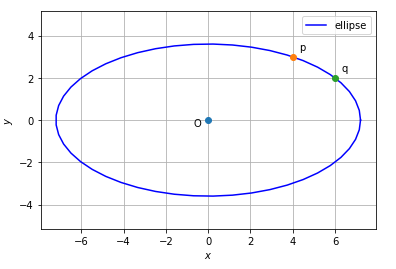
\includegraphics[width=\columnwidth]{solutions/su2021/2/72/k/ellipse(1).PNG}
\caption{Plot of standard ellipse}
\label{quadform/72/k/Plot of standard ellipse}
\end{figure}
The center and axes of the ellipse is given as
\begin{align}
\vec{c} = \vec{0};
\frac{1}{\sqrt{\lambda_1}}  = \sqrt{52},
\frac{1}{\sqrt{\lambda_2}} =\sqrt{13}.
\end{align}
Now let us consider the case when the ellipse is not in the standard form then we have the center to be $\vec{c}=\myvec{\beta\\0}$.The equation is given by:
\begin{align}
(\vec{x}-\vec{c})^{\top}\vec{D}(\vec{x}-\vec{c})=1\label{quadform/72/k/eq:14}
\end{align}
where $\vec{D}$ is a diagonal matrix.
$\because \vec{p}, \vec{q}$ satisfy \eqref{quadform/72/k/eq:14}, we have
\begin{align}
\label{quadform/72/k/eq:ellipse_act_ab}
(\vec{p}-\vec{c})^{\top}\vec{D}(\vec{p}-\vec{c}) &= 1,
\\
(\vec{q}-\vec{c})^{\top}\vec{D}(\vec{q}-\vec{c}) &= 1,
\end{align}
which can be simplified as
\begin{align}
    2\brak{\vec{p}-\vec{q}}^{\top}\vec{D}\vec{c}=\vec{p}^{\top}\vec{D}\vec{p}-\vec{q}^{\top}\vec{D}\vec{q} \label{quadform/72/k/eq:4}
\end{align}
Using the identity,
\begin{align}
   (\vec{p}^{\top}-\vec{q}^{\top})\vec{D}(\vec{p}+\vec{q})
   =\vec{p}^{\top}\vec{D}\vec{p}-\vec{q}^{\top}\vec{D}\vec{q}
\end{align}
in the equation \eqref{quadform/72/k/eq:4}
\begin{align}
    2\brak{\vec{p}-\vec{q}}^{\top}\vec{D}\vec{c}=(\vec{p}-\vec{q})^{\top}\vec{D}(\vec{p}+\vec{q})\\
    \implies (\vec{p}-\vec{q})^{\top}\vec{D}(2\vec{c}-(\vec{p}+\vec{q}))
\end{align}
Thus $\vec{c}$ can be expressed in parametric form as
\begin{align}
\vec{c}=\frac{1}{2}((\vec{p}+\vec{q})+k\vec{D}^{-1}\vec{m}) \label{quadform/72/k/eq:7}
\end{align}
where,
\begin{align}
    (\vec{p}-\vec{q})^{\top}\vec{m}=0 \label{quadform/72/k/eq:6}
\end{align}
and $k$ is a constant.Substituting numerical values in \eqref{quadform/72/k/eq:6}, \begin{align}
    \vec{p}-\vec{q} = \myvec{-2 \\ 1} \implies \vec{m} = \myvec{-1 \\ -2}
\end{align}
and
\begin{align}
    \vec{p}+\vec{q} = \myvec{10 \\ 5}
\end{align}
substituting in \eqref{quadform/72/k/eq:7},we get
\begin{align}
 \myvec{\beta\\0}=\frac{1}{2}\brak{\myvec{10 \\ 5} + k\myvec{\frac{1}{\lambda_1}&0 \\ 0&\frac{1}{\lambda_2}}\myvec{-1 \\ -2}}
\end{align}
From the given information,the X-axis is the major axis.Hence,
\begin{align}
\frac{\lambda_2}{\lambda_1}>1 \implies
    \frac{20-4\beta}{5}>1\\
    \beta<3.75
\end{align}
The possible ellipse satisfying the above conditions are plotted below
\begin{figure}[!ht]
\centering
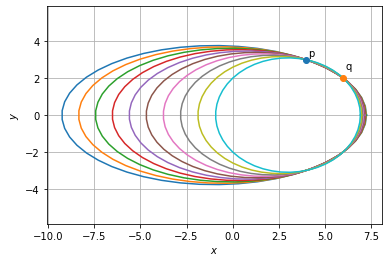
\includegraphics[width=\columnwidth]{solutions/su2021/2/72/k/Ellipse_(I).PNG}
\caption{Ellipses passing through the two points with X axis as major axis}
\label{quadform/72/k/fig:ellipses}	
\end{figure}


\end{enumerate}
%
\item In each of the exercises, find the coordinates of the foci, the vertices, the length of major axis, the minor axis, the eccentricity and the length of the latus rectum of the ellipse.
%
\begin{enumerate}
\item 
$
\vec{x}^T\myvec{\frac{1}{16} & 0 \\ 0 & -\frac{1}{9}}\vec{x} = 1
$
\item 
$
\vec{x}^T\myvec{\frac{1}{9} & 0 \\ 0 & -\frac{1}{27}}\vec{x} = 1
$
%
\item 
$
\vec{x}^T\myvec{9 & 0 \\ 0 & -4}\vec{x} = 36
$
%
\item 
$
\vec{x}^T\myvec{16 & 0 \\ 0 & -9}\vec{x} = 576
$
%
\item 
$
\vec{x}^T\myvec{5 & 0 \\ 0 & -9}\vec{x} = 36
$
\item 
$
\vec{x}^T\myvec{49 & 0 \\ 0 & -16}\vec{x} = 784
$
%
%
\end{enumerate}
\item In each of the following, find the equation for the ellipse that satisfies the given conditions:
%
\begin{enumerate}
\item Vertices $\myvec{\pm 2\\ 0}$, foci $\myvec{\pm 3\\ 0}$ 
\item  Vertices $\myvec{0\\ \pm 5}$, foci $\myvec{0\\ \pm 8}$ 
\item  Vertices $\myvec{ 0\\ \pm 3}$, foci $\myvec{0 \\\pm 5}$ 
\item  Transverse axis length 8, foci $\myvec{\pm 5\\ 0}$.
\item  Conjugate axis length 24, foci $\myvec{0 \\ \pm 13}$.
\item  Latus rectum  length 8, foci $\myvec{ \pm 3\sqrt{5} \\ 0}$.
\item  Latus rectum  lenght 12, foci $\myvec{ \pm 4 \\ 0}$.
\item  Ends of major axis $\myvec{0\\ \pm 5 }$, ends of minor axis $\myvec{\pm 1\\ 0}$ 
\item  Vertices $\myvec{  \pm 7 \\ 0}$, $e = \frac{4}{3}$
\item  Foci $\myvec{ 0\\  \pm \sqrt{10}}$, passing through $\myvec{2\\3}$.

\end{enumerate}

%
\item Find the slope of the tangent to the curve $y = \frac{x-1}{x-2}, x\ne 2$ at $x = 10$.
\\
\solution 
The given curve,
% \begin{align}
% y&=\frac{{x-1}}{{x-2}} 
% \end{align}
 can be expressed as,
\begin{align}
yx-2y-x+1 =0
\label{quadform/75/2.0.1}
\end{align}
yielding
\begin{align}
\vec{V}&=\myvec{\frac{1}{2} & 0 \\ 0 & \frac{1}{2}},\vec{V}^{-1}=\myvec{0&2\\2&0}\vec{u}=\myvec{-\frac{1}{2}\\-1},
f =1 \label{quadform/75/2.0.3}
\end{align}
\begin{align}
\because  |\vec{V}| < 0
\end{align}
 \eqref{quadform/75/2.0.1} is a hyperbola.
Let the slope of tangent be $r$. Then the  direction vector and normal vector of tangent to \eqref{quadform/75/2.0.1} are
\begin{align}
    \vec{m}&= \myvec{1\\r},\vec{n}=\myvec{r\\-1} \label{quadform/75/2.0.5}\\
\kappa=&\pm \sqrt{\frac{\vec{u^T}\vec{V}^{-1}\vec{u}-\vec{f}}{\vec{n^T}\vec{V}^{-1}\vec{n}}}\\
&=\sqrt{\frac{-1}{4r}} \label{quadform/75/2.0.8}
\end{align}
For hyperbola, the point of contact for the tangent is
\begin{align}
\vec{q}&=\vec{V}^{-1}(\kappa\vec{n}-\vec{u})\label{quadform/75/2.0.6}\\
\implies \vec{V}\vec{q}+\vec{u}&=\kappa\vec{n}\\
\implies \myvec{\frac{1}{16}\\4}&=\kappa\vec{n} \quad ( \text{ From } \quad \eqref{quadform/75/2.0.3})\\
\implies \myvec{\frac{1}{16}\\4}&=\sqrt{\frac{-1}{4r}}\myvec{r\\-1}\\
\implies \myvec{\frac{1}{16}\\4}&=\myvec{r\sqrt{\frac{-1}{4r}}\\-\sqrt{\frac{-1}{4r}}}\\
\implies -\sqrt{\frac{-1}{4r}}&=4\\
\implies r &= -\frac{1}{64}
\end{align}
which is the desired slope. Fig.     \ref{quadform/75/fig:Tangent to HYPERBOLA.} verifies this result.
\begin{figure}[!ht]
    \centering
    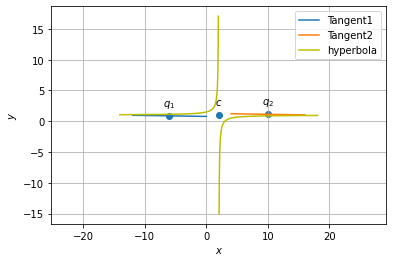
\includegraphics[width=\columnwidth]{solutions/su2021/2/75/HYPERBOLA.png}
    \caption{Tangent to HYPERBOLA.}
    \label{quadform/75/fig:Tangent to HYPERBOLA.}
\end{figure}  



\item Find a point on the curve $y = (x – 2)^2$ at which the tangent is parallel to the chord joining the points \myvec{2\\ 0} and \myvec{4\\ 4}.
\item Find the equation of all lines having slope – 1 that are tangents to the curve $\frac{1}
{x -1}, x \ne 1$
\item Find the equation of all lines having slope 2 which are tangents to the curve $\frac{1}
{x - 3} , x \ne 3$.
%
\\
\solution

Given curve  
\begin{align}
    y &= \frac{1}{x-3} , x \neq 3 \label{quadform/78/giveneq}
    \\
    \implies xy - 3y - 1 &= 0
\end{align}

$\therefore$
\begin{align}
    \vec{V} &= \frac{1}{2}\myvec{0 & 1 \\ 1 & 0}
    \\
    \vec{u} &= \frac{-3}{2}\myvec{0 \\ 1}
    \\
    f &= -1
\end{align}

$\because$
\begin{align}
    \abs{\vec{V}} &= \frac{-1}{4}
    \\
    \implies \abs{\vec{V}} &< 0
\end{align}
$\therefore$ \eqref{quadform/78/giveneq} represents a hyperbola .
Now,the characteristic equation of $\vec{V}$ is 
\begin{align}
    \abs{\vec{V} - \lambda\vec{I}} = \mydet{-\lambda & \frac{1}{2} \\ \frac{1}{2} & -\lambda} &= 0
    \\
    \implies \lambda^2 - \frac{1}{4} &= 0
\end{align}
$\therefore$ Eigen values are 
\begin{align}
    \lambda_1 = \frac{1}{2} , \lambda_2 = \frac{-1}{2}
\end{align}
Eigen vector $\vec{p}$ is 
\begin{align}
    \vec{V}\vec{p} &= \lambda\vec{p}
    \\
    \implies (\vec{V} - \lambda\vec{I})\vec{p} &= 0
\end{align}
Eigen vector $\vec{p}_1$ corressponding to $\lambda_1$ can be obtained as
\begin{align}
    (\vec{V} - \lambda_1\vec{I}) &= \myvec{\frac{-1}{2} & \frac{1}{2} \\ \frac{1}{2} & \frac{-1}{2}}\xleftrightarrow[R_1 \leftarrow -2R_1]{R_2 = R_1 + R_2}\myvec{1 & -1 \\ 0 & 0}
    \\
    \implies \vec{p_1} &= \frac{1}{\sqrt{2}}\myvec{1 \\ 1}
\end{align}
Similarly,
\begin{align}
    \vec{p_2} &= \frac{1}{\sqrt{2}}\myvec{-1 \\ 1}
\end{align}
$\therefore$
\begin{align}
    \vec{P} &= \myvec{\vec{p_1} & \vec{p_2}} = \frac{1}{\sqrt{2}}\myvec{1 & -1 \\ 1 & 1}
    \\
    \vec{D} &= \myvec{\lambda_1 & 0 \\ 0 & \lambda_2} = \myvec{\frac{1}{2} & 0 \\ 0 & \frac{-1}{2}}
\end{align}
Now,
\begin{align}
    \vec{c} &= -\vec{V}^{-1}\vec{u} 
    \\
    &= -\myvec{0 & 2 \\2 & 0}\myvec{0 \\ \frac{-3}{2}}
    \\
    &= \myvec{3 \\ 0}
\end{align}
and
\begin{align}
    \sqrt{\frac{ \vec{u}^T\vec{V}^{-1}\vec{u} - f}{\lambda_1}} &= \sqrt{2}
    \\
    \sqrt{ \frac{f- \vec{u}^T\vec{V}^{-1}\vec{u}}{\lambda_2}} &= \sqrt{2}
\end{align}
$\therefore$ Equation of standard hyperbola can be expressed as 
\begin{align}
    \frac{x^2}{2} - \frac{y^2}{2} &= 1
\end{align}
Now,direction vector of tangent with slope = 2 is
\begin{align}
    \vec{m} &= \myvec{1 \\ m} = \myvec{1 \\ 2}
\end{align}
and,normal vector of same tangent is 
\begin{align}
    \vec{m}^T\vec{n} &= 0
    \\
    \implies \vec{n} &= \myvec{2 \\ -1} 
\end{align}
Now,
\begin{align}
    \kappa &= \pm \sqrt{\frac{\vec{u}^T\vec{V}^{-1}\vec{u}-f}{\vec{n}^T\vec{V}^{-1}\vec{n}}}
    \\
    &= \pm \sqrt{\frac{1}{-8}}
\end{align}
$\therefore$ Real value of $\kappa$ does not exist and hence points of contacts of tangent $\vec{q_1},\vec{q_2}$ also does not exist.
\\
Hence,there exists no tangent to the curve having slope = 2.  The hyperbola is plotted in Fig. \ref{quadform/78/fig:hyperbola}.	
%
\begin{figure}[!ht]
\centering
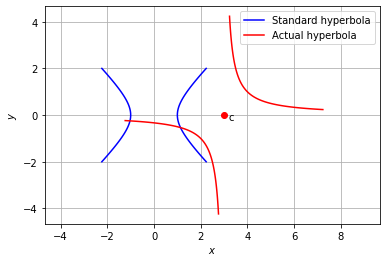
\includegraphics[width=\columnwidth]{solutions/su2021/2/78/Figure8.png}
\caption{Standard and actual hyperbola}
\label{quadform/78/fig:hyperbola}	
\end{figure}



\item Find points on the curve 
$
\vec{x}^T\myvec{\frac{1}{9} & 0 \\ 0 & \frac{1}{16}}\vec{x} = 1
$
%
at which tangents are
\begin{enumerate}
\item  parallel to x-axis
\item  parallel to y-axis.
\end{enumerate}
%
\solution

Given curve,
\begin{align}
\vec{x}^T\myvec{\frac{1}{9} & 0 \\ 0 & \frac{1}{16}}\vec{x} = 1 \label{quad/79/2.0.1}
\end{align}
where,
\begin{align}
\vec{V}&=\myvec{\frac{1}{9} & 0 \\ 0 & \frac{1}{16}},\vec{V}^{-1}=\myvec{9&0\\0&16}\vec{u}=0, f = -1 
\end{align}
\begin{align}
\because |\vec{V}| > 0
\end{align}
given curve \eqref{quad/79/2.0.1} is ellipse.
For an ellipse, the point of contact for the tangent is
\begin{align}
\vec{q}&=\vec{V}^{-1}(\kappa\vec{n}-\vec{u})\\
&=\vec{V}^{-1}\kappa\vec{n}\quad\quad\quad(\because \vec{u}=0). \label{quad/79/2.0.5}
\end{align}
where,
\begin{align}
\kappa=&\pm \sqrt{\frac{\vec{u^T}\vec{V}^{-1}\vec{u}-f}{\vec{n^T}\vec{V}^{-1}\vec{n}}}\\
      =&\pm \sqrt{\frac{-f}{\vec{n^T}\vec{V}^{-1}\vec{n}}}\label{quad/79/2.0.7}\quad \quad\quad(\because \vec{u}=0)
\end{align}
\begin{enumerate}
\item For the tangents  parallel to x-axis, then direction and normal vectors are,
\begin{align}
\vec{m_1} = \myvec{1\\0},\vec{n_1} = \myvec{0\\1},
\kappa_1 &=\pm \sqrt{\frac{-f}{\vec{n_1^T}\vec{V}^{-1}\vec{n_1}}} \\
 &=\pm\frac{1}{4}
\end{align}
$\therefore$ By Substituting $\kappa_1,\vec{n_1},\vec{V}^{-1}$ in \eqref{quad/79/2.0.5}
\begin{align}
\vec{q}&=\vec{V}^{-1}\kappa_1\vec{n_1} \\
&=\myvec{0\\\pm4}
\end{align}
% $\therefore$ Point of contact for tangents of ellipse are,
% \begin{align}
%   \vec{q_1}=\myvec{0\\4},\vec{q_2}=\myvec{0\\-4}
% \end{align}
\item For the tangents  parallel to the y-axis, the direction and normal vectors are
\begin{align}
\vec{m_2} = \myvec{0\\1},\vec{n_2} = \myvec{1\\0},
\kappa_2 &=\pm \sqrt{\frac{-f}{\vec{n_2^T}\vec{V}^{-1}\vec{n_2}}} \\
 &=\pm\frac{1}{3}
\end{align}
$\therefore$ substituting $\kappa_2,\vec{n_2},\vec{V}^{-1}$ in \eqref{quad/79/2.0.5}
\begin{align}
\vec{q}&=\vec{V}^{-1}\kappa_2\vec{n_2} \\
&=\myvec{0\\\pm3}
\end{align}
% $\therefore$ Point of contact for tangents of ellipse are,
% \begin{align}
%   \vec{q_3}=\myvec{3\\0},\vec{q_4}=\myvec{-3\\0}
% \end{align}
\end{enumerate}
The above results are verified in Fig.     \ref{quad/79/fig:Tangent to ELLIPSE.}
%
\begin{figure}[!ht]
    \centering
    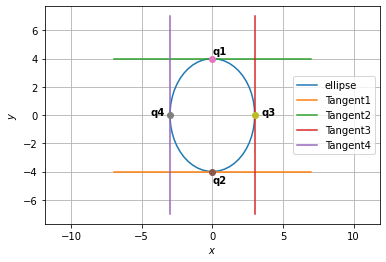
\includegraphics[width=\columnwidth]{solutions/su2021/2/79/ELLIPSE.png}
    \caption{Tangents to ELLIPSE.}
    \label{quad/79/fig:Tangent to ELLIPSE.}
\end{figure}  



\item Find the equations of the tangent and normal to the given curves at the indicated points:
$
y = x^2
$
at \myvec{0\\0}.
\item Find the equation of the tangent line to the curve $y = x^2-2x+7$
\begin{enumerate}
%
\item  parallel to the line $\myvec{2 & -1}\vec{x}= -9$ 
\item  perpendicular to the line $\myvec{-15 & 5}\vec{x} = 13$. 
\end{enumerate}
\item Find the equation of the tangent to the curve $y = \sqrt{3x - 2}$ which is parallel to the line $\myvec{4 & -2}\vec{x}+ 5 =0$ .
%
\solution
The given equation can be expressed as 
\begin{align}
    \vec{x}^{\top}\myvec{0&0 \\ 0&1}\vec{x}+\myvec{-3&0}\vec{x}+2=0 \label{quadform/82/eq:giveneq}
\end{align}
and 
\begin{align}
\therefore \vec{u}=\myvec{\frac{-3}{2} \\ 0}
\\
\vec{V} =\myvec{0&0 \\ 0&1}
\\
\implies {\mydet{\vec{V}}}=0
\end{align}
Thus the curve is a parabola with eigenvalues 
\begin{align}
 \lambda= 0,1
\end{align}
The corresponding  eigenvectors are 
\begin{align}
    \myvec{0&0 \\ 0&1}\vec{x} = 0\implies \vec{p_{1}}= \myvec{1 \\ 0}
    \\
    \myvec{-1&0 \\ 0&0}\vec{x} = \vec{x}\implies \vec{p_{2}}= \myvec{0 \\ 1}
\end{align}
and 
\begin{align}
    \vec{V} = \vec{P}\vec{D}\vec{P}^{\top}\label{quadform/82/eq:eqn1}
\end{align}
where 
\begin{align}
 \vec{P} = \myvec{\vec{p_{1}} & \vec{p_{2}}} = \myvec{1&0 \\ 0&1}
 \\
 \vec{D}=\myvec{\lambda_{1}&0 \\ 0&\lambda_{2}} = \myvec{0&0 \\ 0&1}
\end{align}
Since the given parallel line equation  is 
\begin{align}
 \myvec{4&-2}\vec{x} + 5 = 0, \label{quadform/82/eq:eqn2}
\end{align}
%Now the tangent to the parabola is parallel to the line equation \eqref{quadform/82/eq:eqn2},
the normal vector $\vec{n}$ and the direction vector $\vec{m}$ of the tangent to the parabola are given by 
\begin{align}
    \vec{n}=\myvec{4 \\ -2} \label{quadform/82/eq:eqn5}
    \\
    \vec{m}=\myvec{-2 \\ -4}
\end{align}
The  point of contact for the parabola is given by,
\begin{align}
    \myvec{\vec{u}+\kappa \vec{n}^{\top} \\ \vec{V} }\vec{q} 
    = \myvec{\vec{-f}\\\kappa \vec{n} -\vec{u}}
    \\
  \implies \kappa =\frac{\vec{p_{1}}^{\top}\vec{u}}{\vec{p_{1}}^{\top}\vec{n}}
    =\frac{\myvec{1&0}\myvec{\frac{-3}{2} \\ 0}}{\myvec{1&0}\myvec{4 \\ 2}}
    =\frac{-3}{8}
    \end{align}
and 
\begin{align}
    \myvec{-3&\frac{3}{4} \\ 0&0 \\ 0&1} \vec{q}&= \myvec{-2 \\ 0 \\ \frac{3}{4}}
\end{align}
% Now solving for $\vec{q}$ by removing the zero row and representing as augmented matrix and then converting it to echelon form.
% \begin{align}
%     \myvec{-3&\frac{3}{4}&-2 \\ 0&1&\frac{3}{4}}\xleftrightarrow{R_1\rightarrow \brak{\frac{-1}{3}}R_1} \myvec{1&\frac{-1}{4}&\frac{2}{3} \\ 0&1&\frac{3}{4}}
%     \\
%     \myvec{1&\frac{-1}{4}&\frac{2}{3} \\ 0&1&\frac{3}{4}}\xleftrightarrow{R_1\rightarrow R_1+\frac{1}{4}R_2}\myvec{1&0&\frac{41}{48} \\ 0&1&\frac{3}{4}} \label{quadform/82/eq:eqn3}
% \end{align}
%Hence from the \eqref{quadform/82/eq:eqn3} we get the point of contact to be 
yielding 
\begin{align}
    \vec{q}=\myvec{\frac{41}{48} \\ \frac{3}{4}}
\end{align}
The desired equation of the line is 
%Now $\vec{q}$ is the point on the tangent.Hence the equation of the line can be expressed as 
\begin{align}
    \mathbf{n}^{\top}(\mathbf{x}-\mathbf{q}) &= 0\label{quadform/82/eq:eqn6}
    \\
% \end{align}
% where,
% \begin{align}
% \vec{n}^{\top}\vec{q}
%     =\myvec{4&-2}\myvec{\frac{41}{48} \\ \frac{3}{4}} 
%     \\
%     = \frac{23}{12} \label{quadform/82/eq:eqn4}
% \end{align}
% Hence the equation of the tangent to the curve \eqref{quadform/82/eq:giveneq} parallel to the line \eqref{quadform/82/eq:eqn2} is given by substituting the value of $\vec{n}^{\top}\vec{q}$ and $\vec{n}$ from \eqref{quadform/82/eq:eqn4} and \eqref{quadform/82/eq:eqn5} respectively to the equation \eqref{quadform/82/eq:eqn6} 
% \begin{align}
\implies     \myvec{4&-2}\vec{x}&=\frac{23}{12} \label{quadform/82/eq:eqn7}
\end{align}
which is verified in Fig. \ref{quadform/82/Plot of curve and the lines}.
% Hence \eqref{quadform/82/eq:eqn7} is the equation of the tangent.
% The plot of the figure is given below
%
\begin{figure}[ht]
\centering
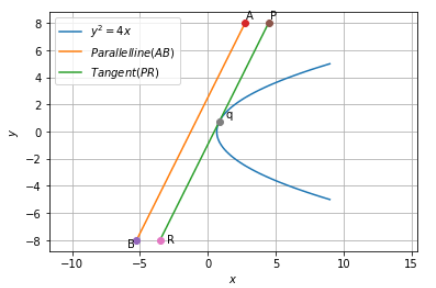
\includegraphics[width=\columnwidth]{solutions/su2021/2/82/Parabola.PNG}
\caption{Plot of curve and the lines}
\label{quadform/82/Plot of curve and the lines}
\end{figure}

\item Find the point at which the line $\myvec{-1 & 1}\vec{x} =  1$ is a tangent to the curve $y^2 = 4x$.
%
\item The line $\myvec{-m & 1}\vec{x} = 1$ is a tangent to the curve $y^2 = 4x$.  Find the value of $m$.
\item  Find the normal at the point \myvec{1\\1} on the curve $2y + x^2 = 3$ 
\item  Find the normal to the curve $x^2=4y$ passing through $\myvec{1\\2}$.
%
\item Find the area of the region bounded by the curve $y^2= x$ and the lines $x = 1, x = 4$ and the x-axis in the first quadrant.
\item  Find the area of the region bounded by $y^2=9x, x=2, x=4$ and the x-axis in the  first quadrant.
%
\item Find the area of the region bounded by $x^2 = 4y, y = 2, y = 4$ and the y-axis in the first quadrant.
\item Find the area of the region bounded by the ellipse 
$
\vec{x}^T\myvec{\frac{1}{16} & 0 \\ 0 & \frac{1}{9}}\vec{x} = 1
$

\item  Find the area of the region bounded by the ellipse 
$
\vec{x}^T\myvec{\frac{1}{4} & 0 \\ 0 & \frac{1}{9}}\vec{x} = 1
$
\item The area between $x=y^2$ and $x=4$ is divided into two equal parts by the line $x=a$, find the value of $a$.
\item  Find the area of the region bounded by the parabola $y = x^2$ and $y = \abs{x}$.
\item  Find the area bounded by the curve $x^2 = 4y$ and the line $\myvec{1 & -1}\vec{x} = -2$.
\item  Find the area of the region bounded by the curve $y^2 = 4x$ and the line $x = 3$.
%
\item Find the area of the region bounded by the curve $y^2 = x$, y-axis and the line $y = 3$.
%
\item Find the area of the region bounded by the two parabolas $y = x^2, y^2=x$.
\item Find the area lying above x-axis and included between the circle $\vec{x}^T\vec{x} -8\myvec{1 & 0}= 0$  and inside of the parabola $y^2 = 4x$.
%
\item AOBA is the part of the ellipse 
$
\vec{x}^T\myvec{9 & 0 \\ 0 & 1}\vec{x} = 36
$
in the first quadrant such that $OA = 2$ and $OB = 6$. Find the area between the arc $AB$ and the chord $AB$.
\\
\solution
Given ellipse is 
\begin{align}
    \vec{x}^T\myvec{9 & 0 \\ 0 & 1}\vec{x} = 36 
\end{align}

On comparing it with standard form
\begin{align}
    \vec{c} &= \myvec{0 \\ 0}
    \\
    \vec{D} &= \myvec{9 & 0 \\ 0 & 1}
    \\
    \vec{u}^T\vec{V}^{-1}\vec{u} - f &= 36
    \\
    \lambda_1 &= 9 
    \\
    \lambda_2 &= 1
\end{align}

$\therefore$  Semi major and minor axes of ellipse are
\begin{align}
    a &= \sqrt{\frac{ \vec{u}^T\vec{V}^{-1}\vec{u} - f}{\lambda_2}} = \sqrt{\frac{36}{1}} = 6
    \\
    b &= \sqrt{\frac{ \vec{u}^T\vec{V}^{-1}\vec{u} - f}{\lambda_1}} = \sqrt{\frac{36}{9}} = 2
\end{align}
$\therefore$ Equation of ellipse can be written as
\begin{align}
    \frac{x^2}{a^2} + \frac{y^2}{b^2} &= 1
    \\
    \implies \frac{x^2}{4} + \frac{y^2}{36} &= 1
\end{align}

Now,area of ellipse is given by
\begin{align}
    A &= \pi ab
    \\
    \implies A &= 12\pi
\end{align}

$\therefore$ Area of a quadrant of ellipse is given by
\begin{align}
    A_1 &= A/4 = 3\pi
\end{align}

Now,from Fig. \ref{quadform/2/99/fig:ellipse} , $AOBA$ is a right angled triangle whose area is given by 
\begin{align}
    A_2 &= \frac{1}{2}ab = 6
\end{align}

$\therefore$ Area between arc $AB$ and chord $AB$ is given by
\begin{align}
    A_3 &= A_1 - A_2 = 3\pi -6
\end{align}


\begin{figure}[!ht]
\centering
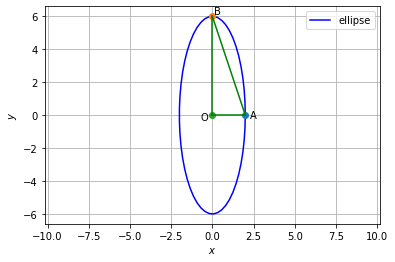
\includegraphics[width=\columnwidth]{solutions/su2021/2/99/Figure7.png}
\caption{Ellipse $\frac{x^2}{4} + \frac{y^2}{36} = 1$}
\label{quadform/2/99/fig:ellipse}	
\end{figure}



\item Find the area lying between the curves $y^2 = 4x$ and $y = 2x$.
\item  Find the area of the region bounded by the curves $y = x^2+2, y = x, x = 0$ and $ x = 3.$
%
\item Find the area under $y = x^2, x = 1, x = 2$ and x-axis.
\item Find the area between  $y = x^2$ and $y = x$.
\item Find the area of the region lying in the first quadrant and bounded by $y = 4x^2, x = 0, y = 1$ and $y = 4$.
\item Find the area enclosed by the parabola $4y = 3x^2$ and the line $\myvec{-3 & 2}\vec{x} = 12$.
%
\\
\solution
\begin{lemma}
The points of intersection of \textbf{Line} $L:\vec{x}=\vec{q}+\mu\vec{m}$ with \textbf{parabola},are given by:
\begin{align}
\vec{x}_i = \vec{q}+\mu_i\vec{m}
\end{align}
%
where,
\begin{multline}
\mu_i = \frac{1}
{
\vec{m}^T\vec{V}\vec{m}
}
\lbrak{-\vec{m}^T\brak{\vec{V}\vec{q}+\vec{u}}}
\\
\pm
{\small
\rbrak{\sqrt{
\sbrak{
\vec{m}^T\brak{\vec{V}\vec{q}+\vec{u}}
}^2
-
\brak
{
\vec{q}^T\vec{V}\vec{q} + 2\vec{u}^T\vec{q} +f
}
\brak{\vec{m}^T\vec{V}\vec{m}}
}
}
}\label{quadform/2/105/eq:mu_i}
\end{multline}
\end{lemma}
 The matrix parameters of the parabola are
\begin{align}
\vec{V}=\myvec{1&0\\0&0},\vec{u}=\myvec{0\\-\frac{2}{3}},f=0 \label{quadform/2/105/eq:v}
\end{align}
with eigen parameters 
\begin{align}
\lambda_1 &= 0 , \lambda_2 = 1
\\
\vec{p_1} &= \myvec{0 \\ 1},
\vec{p_2} = \myvec{1 \\ 0}
\end{align}
The vertex of the parabola can be expressed as
\begin{align} \myvec{\vec{u^T}+\eta\vec{p_1^T}\\\vec{V} }\vec{c} &= \myvec{\vec{-f}\\\eta \vec{p_1} -\vec{u}}
\\
\text{where, }  \eta = \vec{u^T}\vec{p_1} = \frac{-2}{3}
\\
\implies\myvec{0 & \frac{-4}{3}\\1 & 0 \\0 & 0} \vec{c}&= \myvec{0\\0\\0}
\\
\text{or, }
   \vec{c} &= \myvec{0 \\ 0}
\end{align}
From  \eqref{quadform/2/105/eq:mu_i},
\begin{align}
\mu_i &= \frac{1}{4}
\brak{10}
\pm{6}
\\
\implies \mu_1 &= 1, \mu_2 =4
\end{align}
The given line is
\begin{align} 
\myvec{-3&2}\vec{x}&=12
\end{align}
 In parametric form, the given  line can be written as:
\begin{align} 
L: \vec{x}&=\vec{q}+\mu\vec{m}
\\
\implies \vec{x}&=\myvec{-4\\0}+\mu\myvec{2\\3} \label{quadform/2/105/eq:q}
\end{align}
Substitutuing $\mu_1$ and $\mu_2$ in \eqref{quadform/2/105/eq:q},the points of intersection
\begin{align}
 \vec{K}= \myvec{-2\\3},  
\vec{L}&= \myvec{4\\12}
\end{align}

\begin{enumerate}
  \item Thus, from Fig. \ref{quadform/2/105/Plot of the Parabola and line} the area enclosed by parabola and line can be given as
\begin{align}
   A&= \text{Area under line} - \text{Area under parabola}
     \\
   A&= Ar(KLMNK)-Ar(KCLMCNK)
    \\
    A&= A_1 -A_2 \label{quadform/2/105/eqAREA}
    \end{align}
\item Area under the line 2y=3x+12 i.e, $A_1$-
\begin{align}
  A_1&= \int_{-2}^{4} y dx
    \\
    A_1&= \frac{1}{2}\int_{-2}^{4} \brak{3x+12} dx
    \end{align}
    \begin{align}
    A_1= \frac{3}{2}\int_{-2}^{4} x+\frac{1}{2}\int_{-2}^{4}12 dx
    \end{align}
    \begin{align}
    A_1&= \frac{3}{4}\brak{4^2-2^2} +\frac{12}{2}\brak{4+2}
   \\
    A_1&= \frac{3}{4}\brak{12} +\frac{12}{2}\brak{6}
    \\
    A_1&= 9 +36
    \\
    A_1 &=45 \text{ units} \label{quadform/2/105/eqB}
\end{align}
\item Area under the parabola that is $A_2$-
\begin{align}
    A_2&= \int_{-2}^{4} y dx
    \\
    A_2&= \int_{-2}^{4} \frac{3}{4} x^2 dx
    \\
    A_2&= \frac{3}{4} \int_{-2}^{4}  x^2 dx
    \\
    A_2&= \frac{3}{4\times3} \brak{4^3-\brak{-2}^3}
    \\
    A_2&= \frac{1}{4} \brak{64 +8}
    \\
    A_2&= \frac{72}{4} 
    \\
    A_2&= 18 \text{ units} \label{quadform/2/105/eqC}
\end{align}
\item Putting \eqref{quadform/2/105/eqB} and \eqref{quadform/2/105/eqC} in \eqref{quadform/2/105/eqAREA} we get required area A as:
\begin{align}
 A &= A_1 -A_2 
 \\
 A &= 45-18
 \\
 A &= 27 \text{ units}
\end{align}
%
\end{enumerate}
\begin{figure}[ht]
\centering
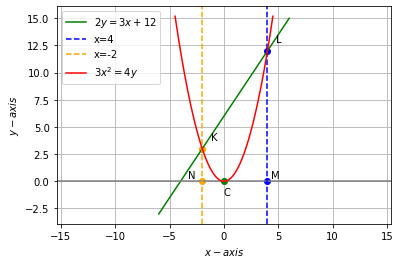
\includegraphics[width=\columnwidth]{solutions/su2021/2/105/LINE AND PARABOLA.png}
\caption{Plot of the parabola and line}
\label{quadform/2/105/Plot of the Parabola and line}
\end{figure}

\item Find the area of the smaller region bounded by the ellipse
$
\vec{x}^T\myvec{\frac{1}{9} & 0 \\ 0 & \frac{1}{4}}\vec{x} = 1
$
and the line 
$
\myvec{\frac{1}{a} & \frac{1}{b}}\vec{x} = 1
$
\item Find the area of the region enclosed by the parabola $x^2=y$, the line $\myvec{-1 & 1}\vec{x} = 2$ and the x-axis.
%
\item Find the area bounded by the curves
\begin{align}
\cbrak{\brak{x,y} : y > x^2, y = \abs{x}}
\end{align}
%
\item Find the area of the region
\begin{align}
\cbrak{\brak{x,y} : y^2 \le 4x, 4\vec{x}^T\vec{x} = 9}
\end{align}
%
\item Find the area of the circle $\vec{x}^T\vec{x} = 16$ exterior to the parabola $y^2 = 6$.
%
\item Find the intervals in which the function given by 
\begin{align}
f(x)  = 2x^2-3x
\end{align}
%
is 
\begin{enumerate}
\item increasing
\item decreasing.
\end{enumerate}
%
\item Find the intervals in which the following functions are strictly increasing or decreasing
%
\begin{enumerate}
\item $x^2+2x-5$
\item $10-6x-2x^2$
\item $6-9x-x^2$
\end{enumerate}
%
\item Prove that the function $f$ given by $f(x) = x^2-x+1$ is neither strictly increasing nor decreasing on $\brak{1,-1}$.
%%
%\item Find the maximum and minimum values, if any, of the following functions given by 
%%
%\begin{enumerate}
%\item $f(x) = \brak{2x-1}^2+3$
%\item $f(x) = 9x^2+12x+2$
%\item $f(x) = -\brak{x-1}^2+10$
%\item $f(x) = x^2$.
%\end{enumerate}
%\item Find the absolute maximum and absoute minimum value of the following functions in the given intervals
%%
%\begin{enumerate}
%\item $f(x) = 4x - \frac{1}{2}x^2, x \in \brak{-2,\frac{9}{2}}$
%\item $f(x) = \brak{x-1}^2 + 3,  x \in \brak{-3,1}$
%\end{enumerate}
%%
%\item Find the maximum profit that a company can make, if the profit function is given by
%\begin{align}
%p(x) = 41-72x - 18x^2
%\end{align}
%%
%\item Find the point on the curve $x^2=2y$ which is nearest to the point $\myvec{0\\5}$.
%\item Find the maximum area of an isosceles triangle inscribed in the ellipse 
%%
%\begin{align}
%\vec{x}^T\myvec{a^2 & 0 \\ 0 & b^2}\vec{x} = a^2b^2
%\end{align}
%%
%with its vertex at one end of the major axis.
%
\item Examine the continuity of the function $f(x) = 2x^2– 1$ at $x = 3$.
\item Find all points of discontinuity of $f$, where $f$is defined by
\begin{align}
f(x)=
\begin{cases}
x+1, & x \ge 1,
\\
x^2+1, & x < 1,
\end{cases}
\end{align}
%
\item For what value of $\lambda $is the function defined by 	
%
\begin{align}
f(x)=
\begin{cases}
\lambda\brak{x^2-2x}, & x \le 0,
\\
4x+1, & x > 0
\end{cases}
\end{align}
%
continuous at $x = 0$? What about continuity at $x = 1$?\item For what value of $k$ is the following function 
%
continuous at the given point.
\begin{align}
f(x)=
\begin{cases}
kx^2, & x \le 2,
\\
3, & x > 2,
\end{cases}
\quad x =2
\end{align}
%
\item Find $\frac{dy}{dx}$ in the following
\begin{align}
x^2 +xy + y^2 = 100
\end{align}
%
\item Verify Rolle's theorem for the function 
\label{prob:conics_ex_eq_rolle}.
$
f(x) = x^2+2x-8, x \in \sbrak{-4,2}
$
\item Examine if Rolle's theorem is applicable to the following function
$
f(x) = x^2-1, x \in \sbrak{1,2}.
$
Can you say some thing about the converse of Rolle's theorem from this example?
\item  Examine the applicability of the mean value theorem for the  function in Problem \ref{prob:conics_ex_eq_rolle}.
%
\item Find $\lim_{x\to 1} \pi r^2$.
%
\item Find $\lim_{x\to 0} f(x)$ where
\begin{align}
f(x) = 
\begin{cases}
x^2-1 & x \le 1
\\
-x^2-1, & x > 1
\end{cases}
\end{align}
%
\item For some constans $a$ and $b$, find the derivative of
%
\begin{align}
\brak{x-a}\brak{x-b}
\end{align}
%
%
\item Integrate the following as limit of sums:
\begin{enumerate}[label = (\roman*)]
\item $\int_{2}^{3}x^2\, dx$
\item $\int_{1}^{4}\brak{x^2-x}\, dx$
\end{enumerate}
\item Form the differential equation of the family of parabolas having vertex at origin and axis along positive y-axis.
\item  Form the differential equation of the family of ellipses having foci on y-axis and centre at origin.
\item  Form the differential equation of the family of hyperbolas having foci on x-axis and centre at origin.
\item The ceiling of a long hall is 25 m high. What is the maximum horizontal distance that a ball thrown with a speed of 40 $m s^{-1}$
can go without hitting the ceiling of the hall ?
\item  A cricketer can throw a ball to a maximum horizontal distance of 100 m. How much high above the ground can the cricketer throw the same ball ?
\item  Find the normal to the curve $x^2=4y$ passing through $\myvec{1\\2}$.
%
\item Find the area of the region bounded by the curve $y^2= x$ and the lines $x = 1, x = 4$ and the x-axis in the first quadrant.
\item  Find the area of the region bounded by $y^2=9x, x=2, x=4$ and the x-axis in the  first quadrant.
%
\item Find the area of the region bounded by $x^2 = 4y, y = 2, y = 4$ and the y-axis in the first quadrant.
\item Find the area of the region bounded by the ellipse 
$
\vec{x}^T\myvec{\frac{1}{16} & 0 \\ 0 & \frac{1}{9}}\vec{x} = 1
$

\item  Find the area of the region bounded by the ellipse 
$
\vec{x}^T\myvec{\frac{1}{4} & 0 \\ 0 & \frac{1}{9}}\vec{x} = 1
$
\item The area between $x=y^2$ and $x=4$ is divided into two equal parts by the line $x=a$, find the value of $a$.
\item  Find the area of the region bounded by the parabola $y = x^2$ and $y = \abs{x}$.
\item  Find the area bounded by the curve $x^2 = 4y$ and the line $\myvec{1 & -1}\vec{x} = -2$.
\item  Find the area of the region bounded by the curve $y^2 = 4x$ and the line $x = 3$.
%
\item Find the area of the region bounded by the curve $y^2 = x$, y-axis and the line $y = 3$.
%
\item Find the area of the region bounded by the two parabolas $y = x^2, y^2=x$.
\item Find the area lying above x-axis and included between the circle $\vec{x}^T\vec{x} -8\myvec{1 & 0}= 0$  and inside of the parabola $y^2 = 4x$.
%
\item AOBA is the part of the ellipse 
$
\vec{x}^T\myvec{9 & 0 \\ 0 & 1}\vec{x} = 36
$
in the first quadrant such that $OA = 2$ and $OB = 6$. Find the area between the arc $AB$ and the chord $AB$.
\item Find the area lying between the curves $y^2 = 4x$ and $y = 2x$.
\item  Find the area of the region bounded by the curves $y = x^2+2, y = x, x = 0$ and $ x = 3.$
%
\item Find the area under $y = x^2, x = 1, x = 2$ and x-axis.
\item Find the area between  $y = x^2$ and $y = x$.
\item Find the area of the region lying in the first quadrant and bounded by $y = 4x^2, x = 0, y = 1$ and $y = 4$.
\item Find the area enclosed by the parabola $4y = 3x^2$ and the line $\myvec{-3 & 2}\vec{x} = 12$.
%
\item Find the area of the smaller region bounded by the ellipse
$
\vec{x}^T\myvec{\frac{1}{9} & 0 \\ 0 & \frac{1}{4}}\vec{x} = 1
$
and the line 
$
\myvec{\frac{1}{a} & \frac{1}{b}}\vec{x} = 1
$
\item Find the area of the region enclosed by the parabola $x^2=y$, the line $\myvec{-1 & 1}\vec{x} = 2$ and the x-axis.
%
\item Find the area bounded by the curves
\begin{align}
\cbrak{\brak{x,y} : y > x^2, y = \abs{x}}
\end{align}
%
\item Find the area of the region
\begin{align}
\cbrak{\brak{x,y} : y^2 \le 4x, 4\vec{x}^T\vec{x} = 9}
\end{align}
%
\item Find the area of the circle $\vec{x}^T\vec{x} = 16$ exterior to the parabola $y^2 = 6$.
\item Find the equation of the circle passing through \myvec{0\\0} and making intercepts a and b on the coordinate axes.
\item Find the locus of all the unit vectors in the xy-plane.
\item Find the area lying in the first quadrant and bounded by the circle $\vec{x}^T\vec{x}=4$ and the lines $x = 0$ and $x = 2$.
%
\item Find the area of the circle $4\vec{x}^T\vec{x}=9$.
\item  Find the equation of the tangent to the curve,
\begin{align}
y = \sqrt{3x-2}
\label{eq:solutions/conics/1/19/Q}
\end{align}
 which is parallel to the line,
\begin{align}
\myvec{4&2}\vec{x}+5=0
\label{eq:solutions/conics/1/19/P}
\end{align}  
\item Find the equations of the tangent and normal to the given curves at the indicated points:
$
y = x^2
$
at \myvec{0\\0}.
\item The line 
\begin{align}
\myvec{-m & 1}\vec{x} = 1 \label{eq:solutions/conics/3/2/21/eq: 1}
\end{align}
is a tangent to the curve $y^2 = 4x$. Find the value of m.
%\end{enumerate}
